\section{Reverberation}
\gls{reverb} is an effect where the sound wave is reflected, and therefore the reflected waves haves another travelling time to the receiver than the sound that is going the direct way. This effect is a very frequently effect which happens each time sound can be reflected by walls, trees, table etc. The following \autoref{fig:reverb_reflect} shows the \gls{reverb} effect form one person to another person \citep{reverb_expl}.

\begin{figure} [htbp]
 \centering
  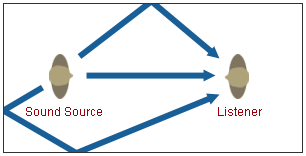
\includegraphics[width=0.7\textwidth]{reverb_reflect}
  \caption{The photo shows a echo in time domain}
  \label{fig:reverb_reflect}
\end{figure}



